\section{Analysis}
\label{Analysis}
After constructing the script and executing it, the following findings were made:\\
0 WST\\
1 MST\\
5 SST\\
A p-value of 0.1414.\\
The p-value is above 0.1 which indicates that the preference tree model is not significant worse than a theoretical perfect model.
In a preference tree model there is both scale values for the stimuli presented in the study, and the attributes the tree is made with. 
The scale values of the attributes is used to illustrate the perceived difference of how big a health risk the substance is, eg. longer branch bigger perceived risk. 
On \autoref{fig:Tree} the preference tree is illustrated with the scale values, and the numbers at each branch is a indicator for the belonging attribute. 
The \textcolor{xGreen}{green} line is modified so it is three times shorter than it normally would be the \textcolor{xRed}{red} is also modified, but it is shortened ten times.
This is done to ensure that all the trees proportions are viewable at the same time.
%The lines on the tree indicates the different attributes that the stimuli have.
\begin{figure}[H]
	\centering
	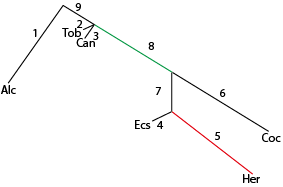
\includegraphics[resolution=300,scale=0.75]{/Tree}
	\caption{}
	\label{fig:Tree}
\end{figure}
\noindent
From the tree it's clear that the different attributes have different effects on how big the perceived health risk is. With these results it's found interesting to investigate how the attributes compare with each other. To compare the attributes the scale values for every branch of the tree is plotted, with the belonging 95\% confidence interval, see \autoref{fig:att}.
\begin{figure}[H]
	\centering
	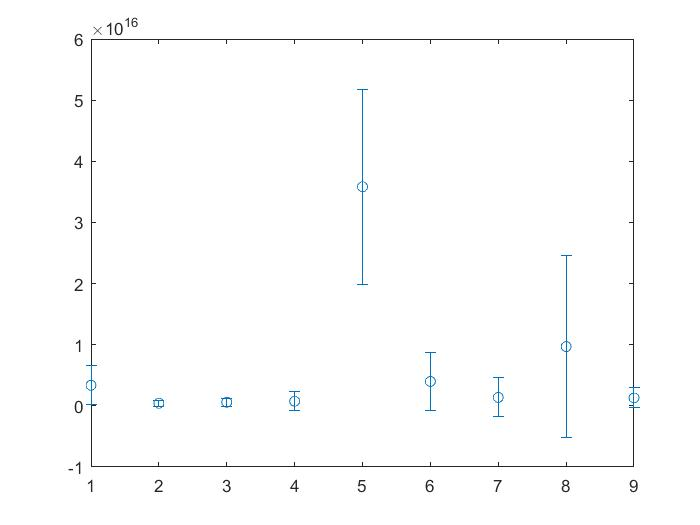
\includegraphics[resolution=300,scale=2]{/att}
	\caption{}
	\label{fig:att}
\end{figure}
\noindent
It's found that the only attribute that is significant different from the others is the cocaine, which is the one that have cocaine at the end.